\documentclass[12pt]{article}
\usepackage{spikey}
\usepackage{amsmath}
\usepackage{amssymb}
\usepackage{soul}
\usepackage{float}
\usepackage{graphicx}
\usepackage{hyperref}
\usepackage{xcolor}
\usepackage{chngcntr}
\usepackage{centernot}
\usepackage{datetime}
\usepackage[shortlabels]{enumitem}

% Set font.
%\usepackage{mathptmx}
\usepackage[MnSymbol]{mathspec}
\setallmainfonts{Times New Roman}

\usepackage[margin=1truein]{geometry}
\usepackage{setspace}
\linespread{1.15}

\counterwithin{equation}{section}
\counterwithin{theorem}{section}
\counterwithin{lemma}{section}
\counterwithin{corollary}{section}
\counterwithin{proposition}{section}
\counterwithin{remark}{section}
\counterwithin{example}{section}
\counterwithin{definition}{section}

% Bib package
\usepackage{apacite}

\title{Title \footnote{Compile Date: \currenttime\ \today}}

\author{Tianyu Du \footnote{\texttt{tianyu.du@mail.utoronto.ca}}}

\begin{document}
	\maketitle
	\tableofcontents
	\newpage

	\section{Missing Data}
	\par
 
	\section{Day of the Week Effect}
	\par \cite{Hess1981}
	\par The following figures present distributions of crude oil returns computed using
	\begin{align}
		r_t &:= \ln(p_t) - \ln(p_{t - \Delta})
	\end{align}
	where $t - \Delta$ is the last trading day before day $t$. For instance, if $t$ is a Monday, then $r_t$ computes the crude oil return between the close price on Monday and the close price on Friday.
	\begin{figure}[H]
		\center
		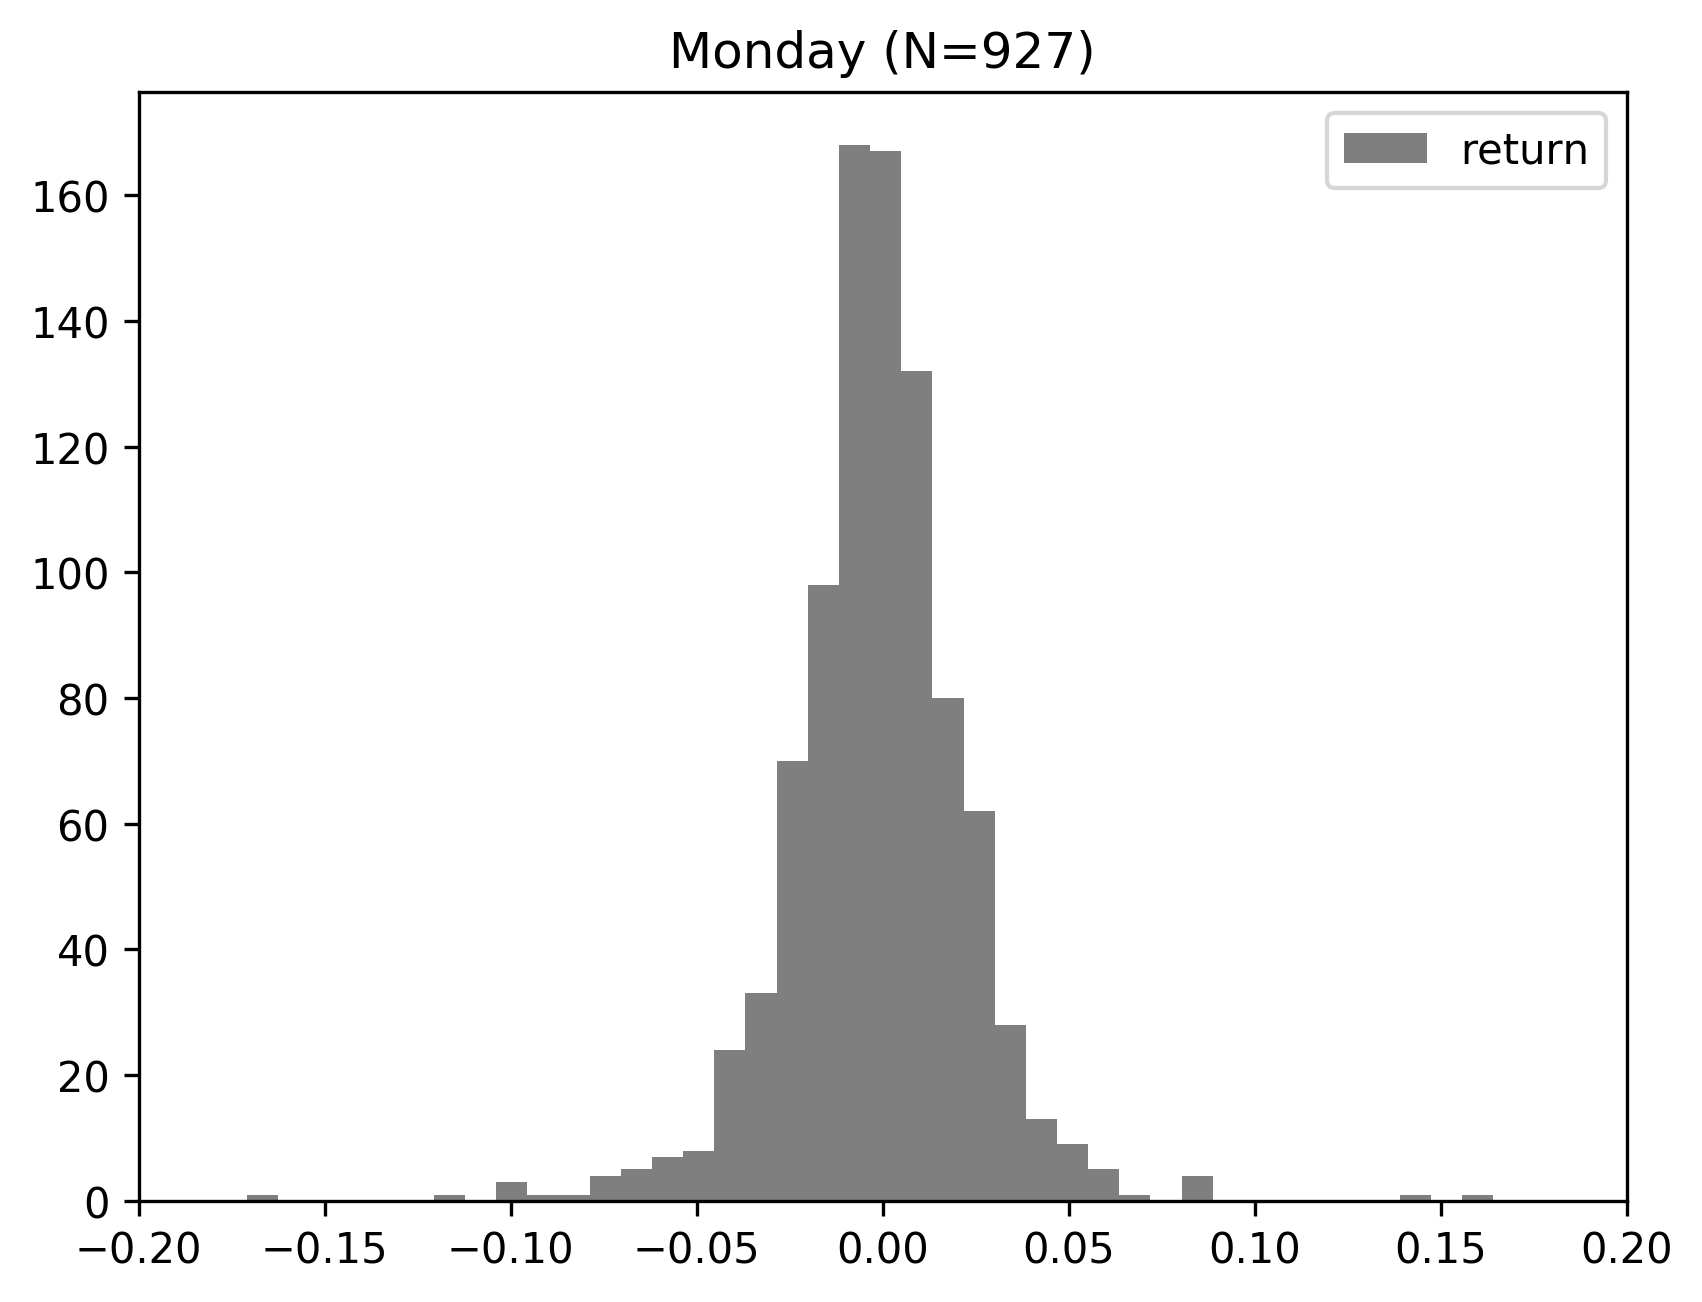
\includegraphics[width=0.45\linewidth]{figures/day_of_week_effect/dist_returns_Monday.png}
		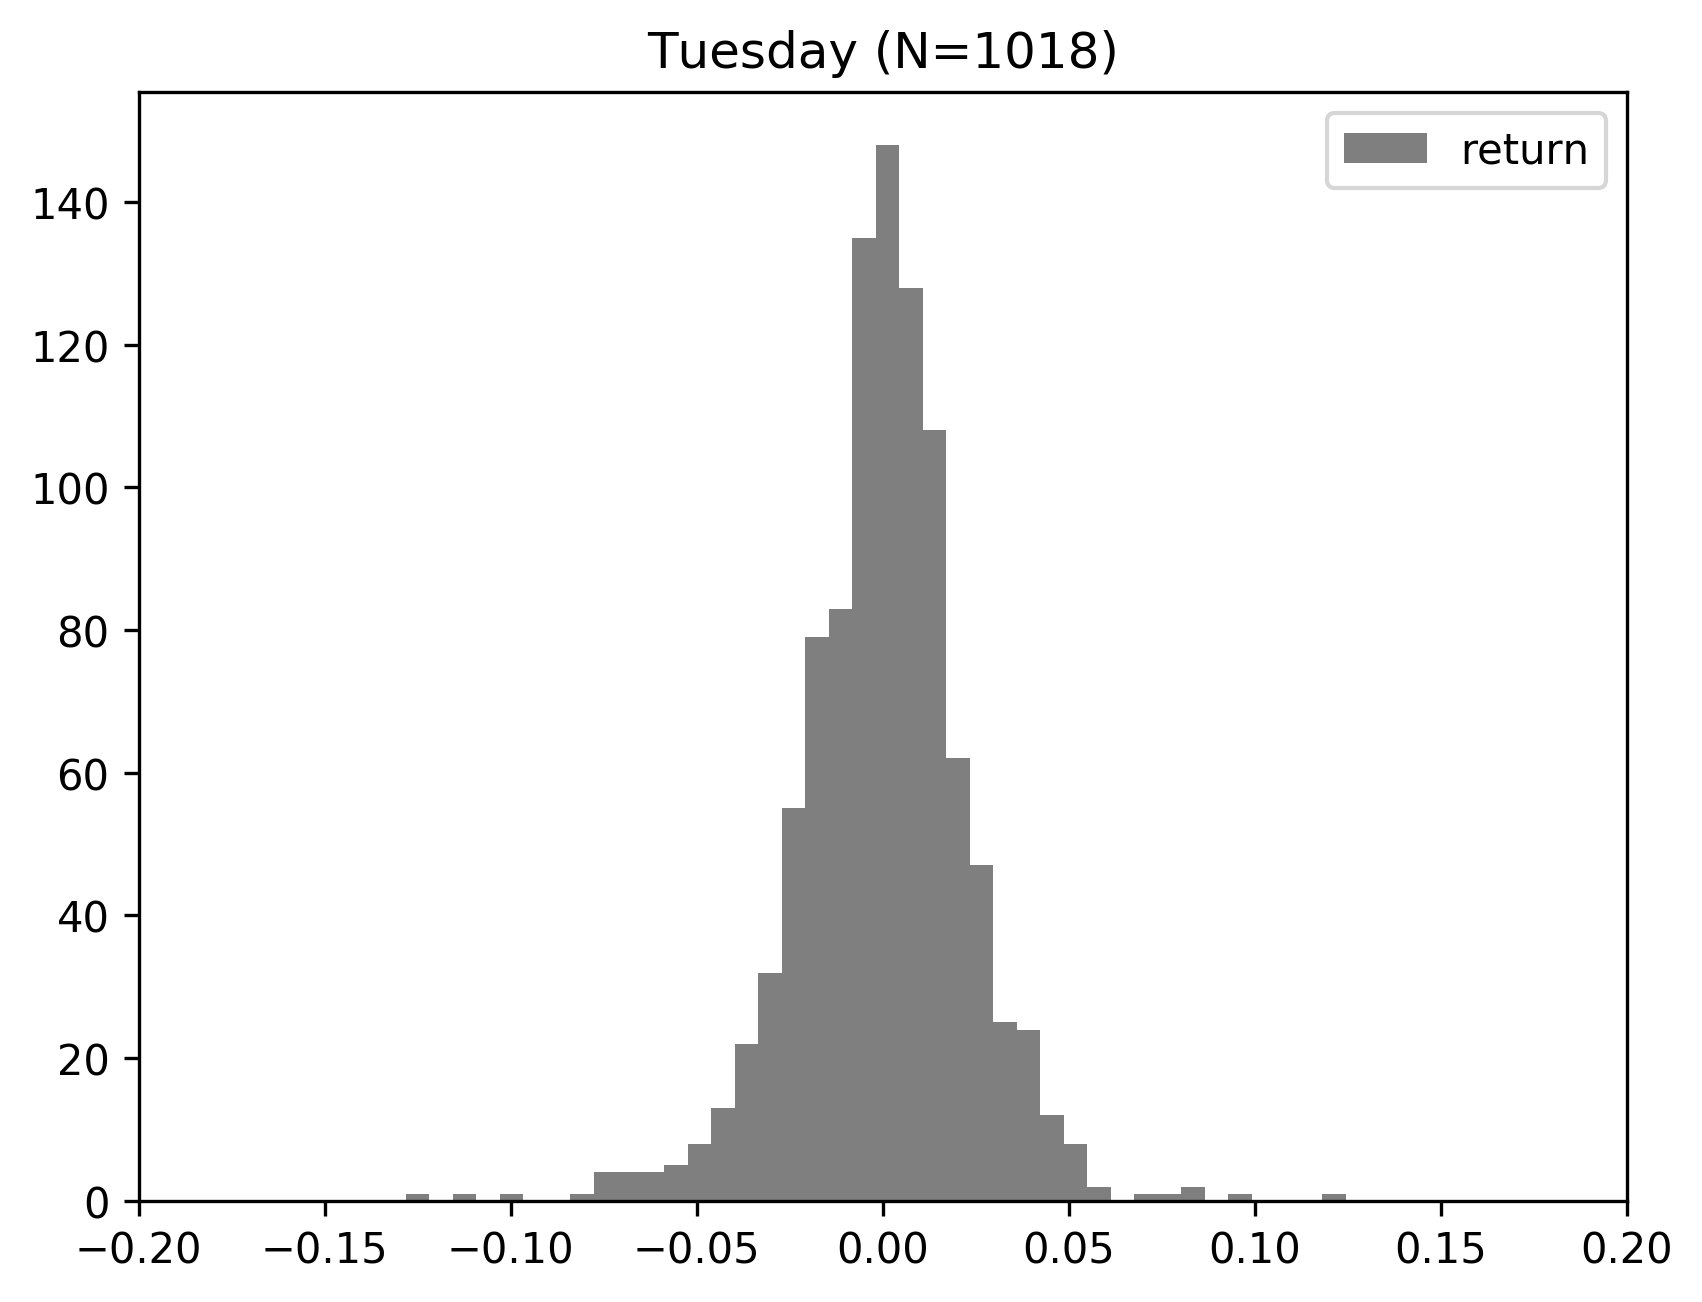
\includegraphics[width=0.45\linewidth]{figures/day_of_week_effect/dist_returns_Tuesday.png}
		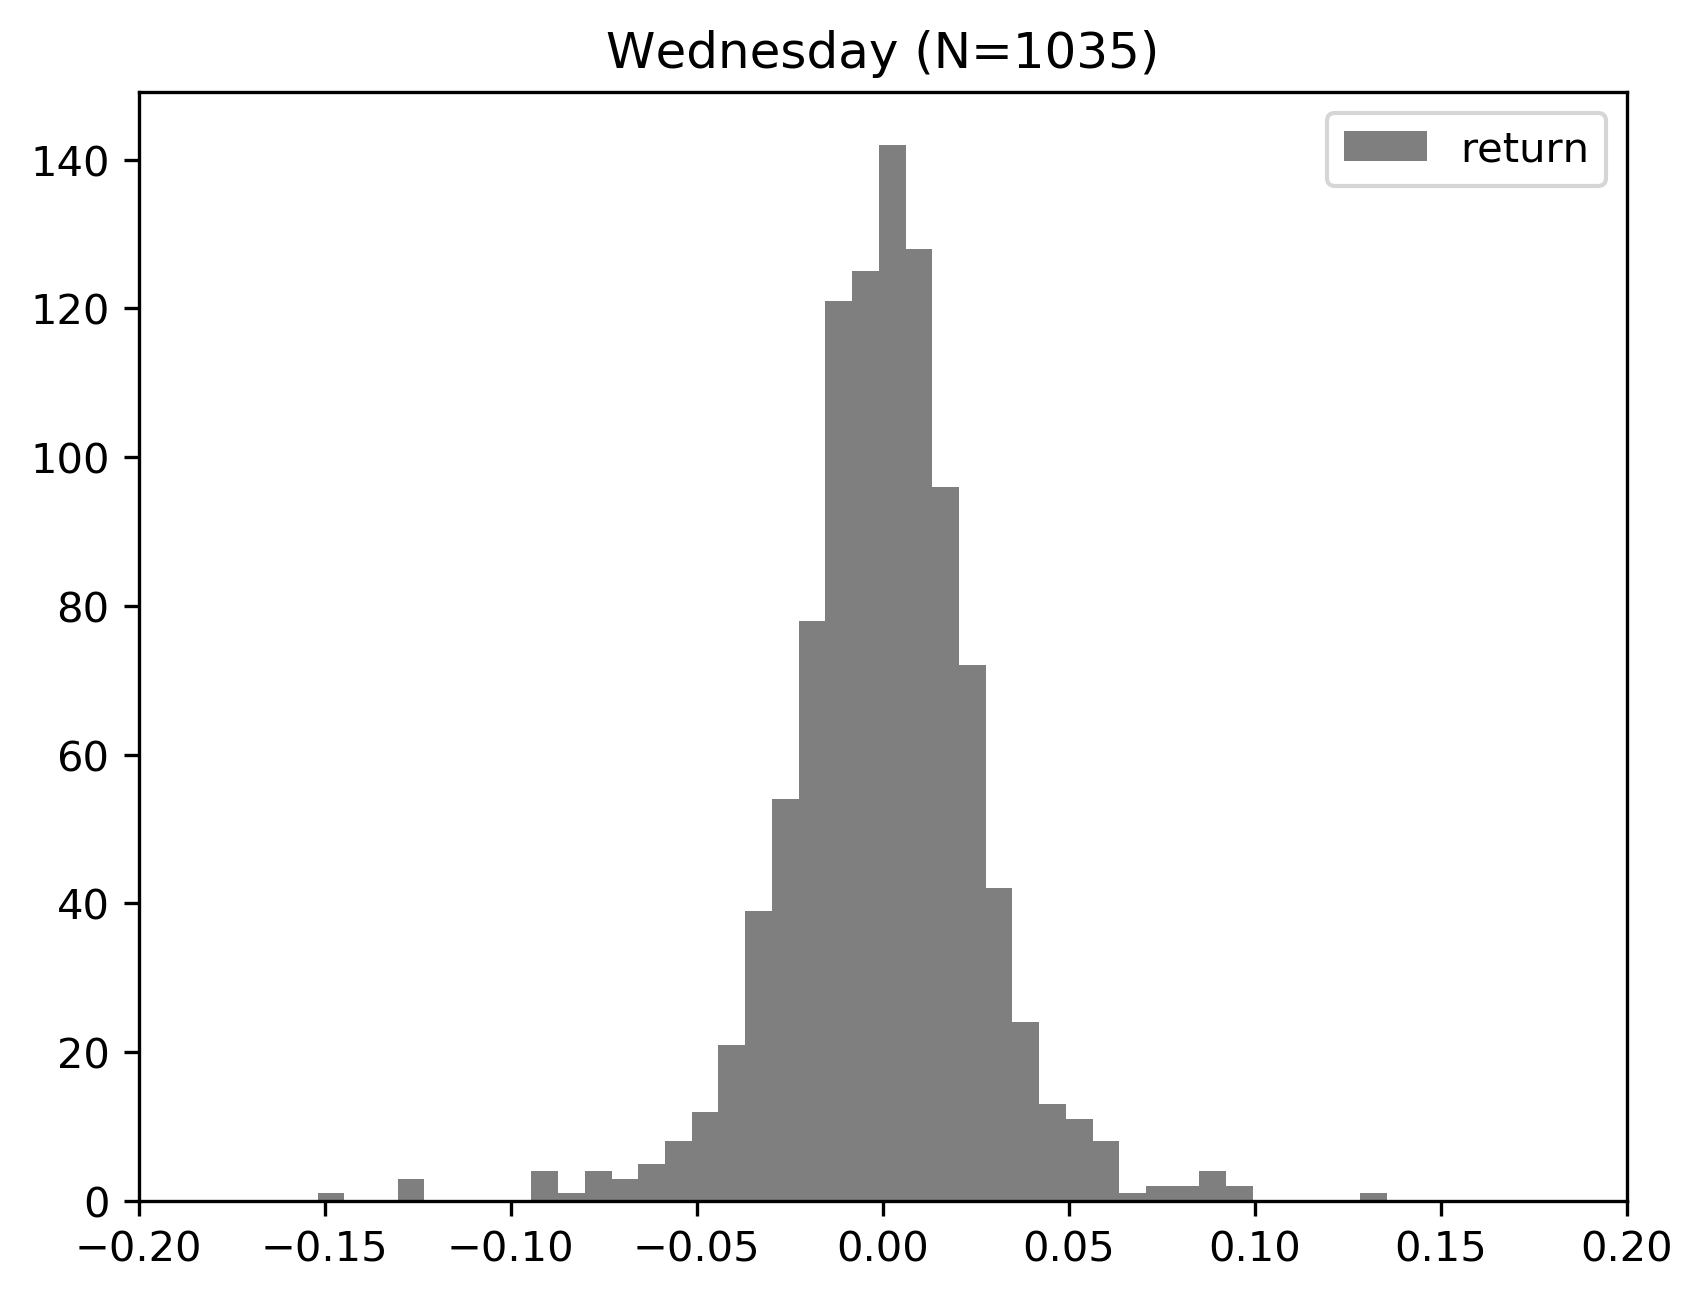
\includegraphics[width=0.45\linewidth]{figures/day_of_week_effect/dist_returns_Wednesday.png}
		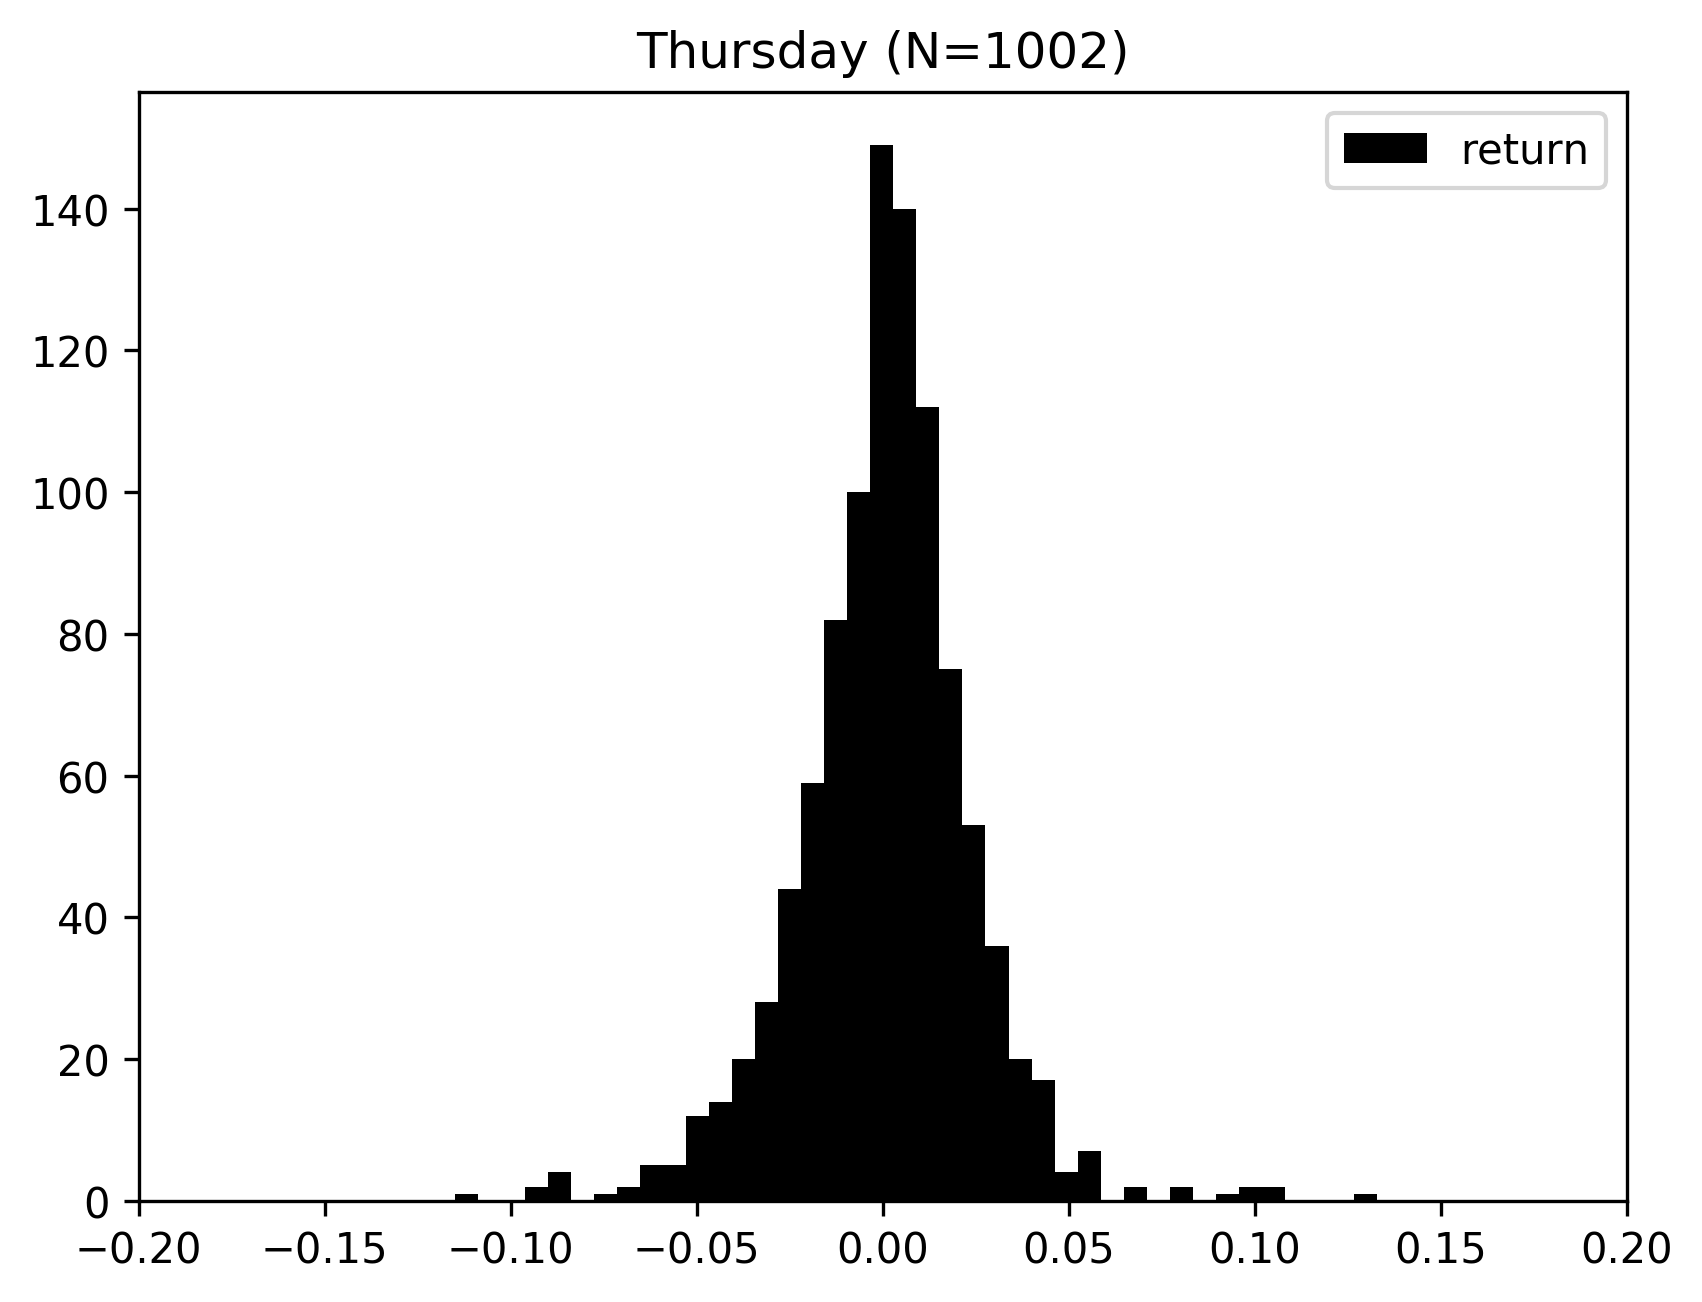
\includegraphics[width=0.45\linewidth]{figures/day_of_week_effect/dist_returns_Thursday.png}
		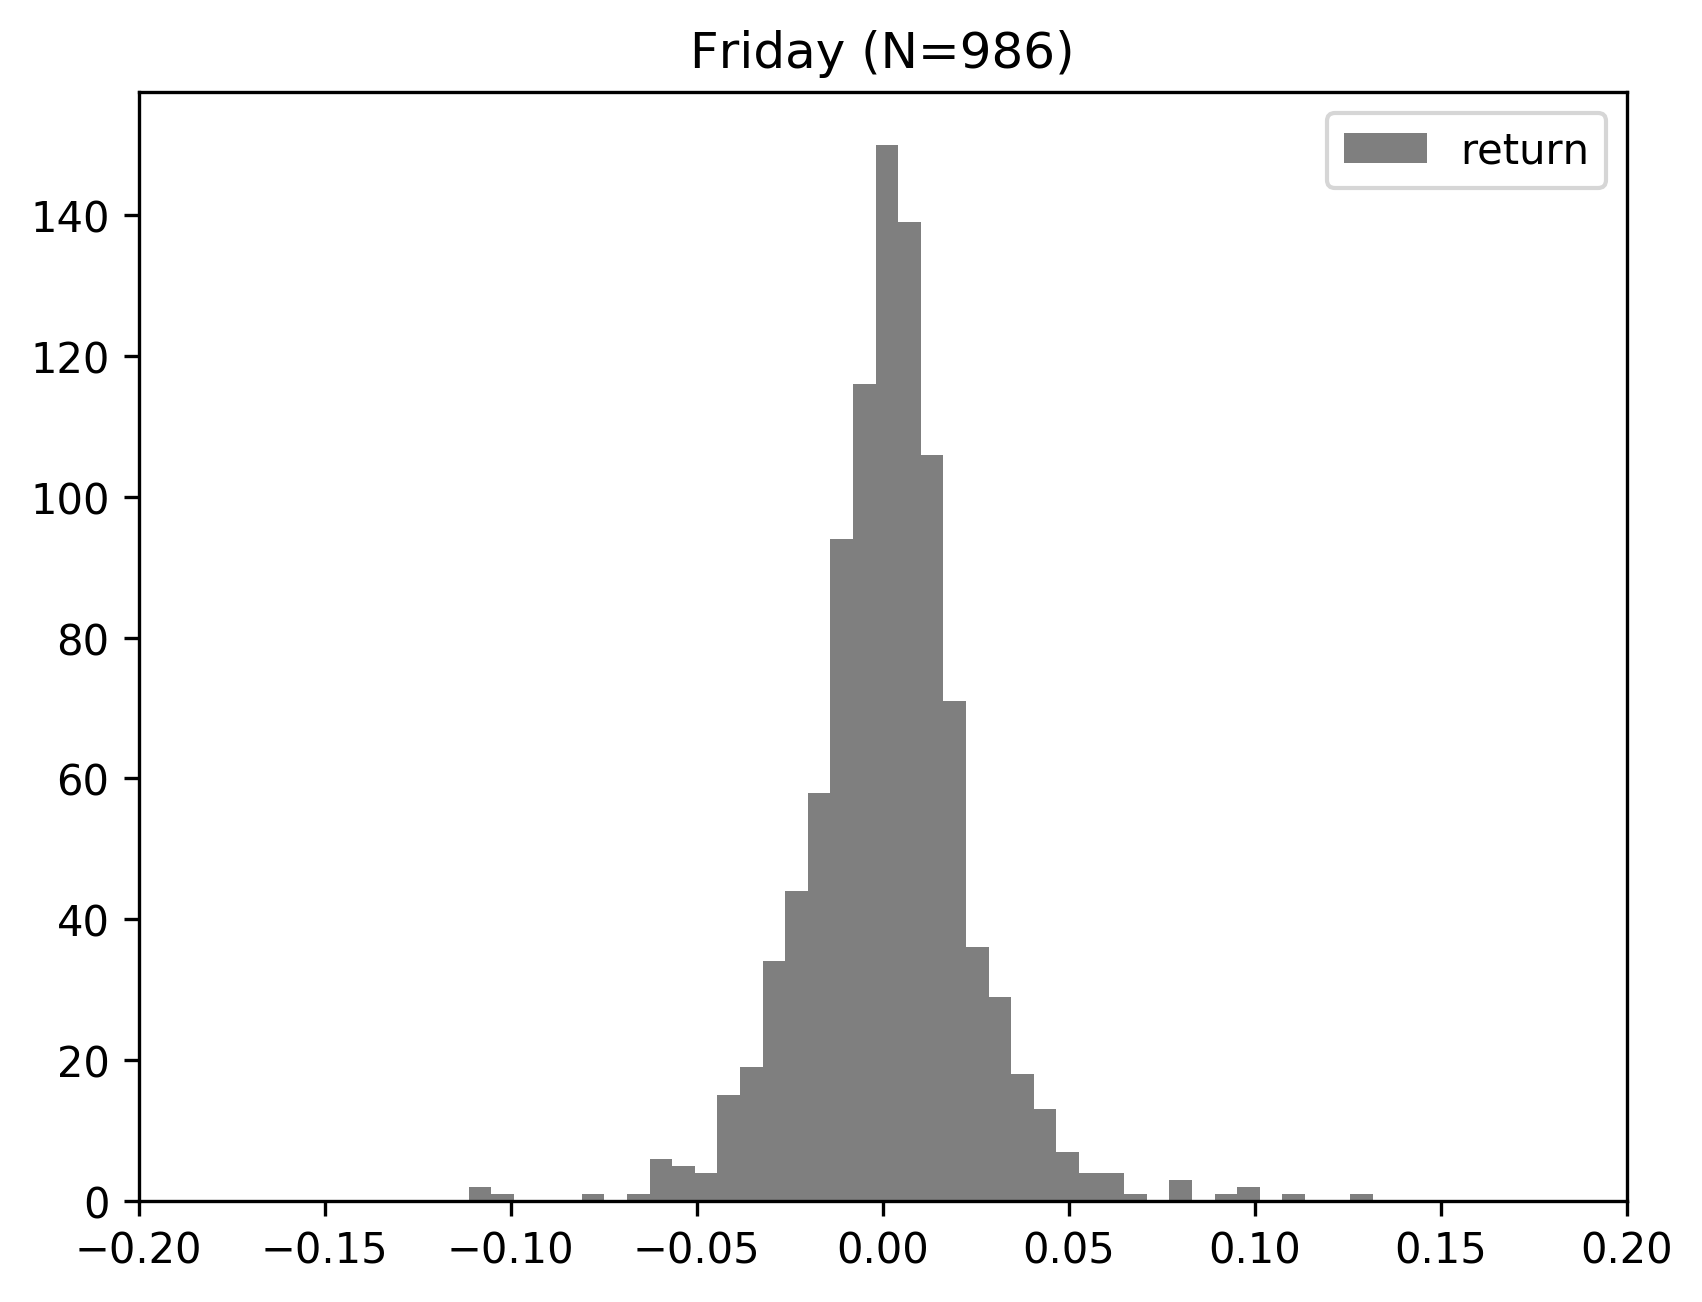
\includegraphics[width=0.45\linewidth]{figures/day_of_week_effect/dist_returns_Friday.png}
		\caption{Crude oil returns on each weekday. Weekend data are not available in the daily dataset provided by EIA. The range of y-axis in all five histograms are from -0.2 to 0.2. $N$s in parentheses denote the number of observations.}
	\end{figure}

	\begin{table}[H]
		\center
		\begin{tabular}{|c|c|c|c|c|}
			\hline
			Day of the week & Num. Obs. & Mean & Std. & $3^{rd}$ Moment \\
			\hline \hline \\
		\end{tabular}
		\caption{}
	\end{table}


	% Bib
	\bibliographystyle{apacite}
	
	\bibliography{thesis.bib}

\end{document}






















